\section{Deep Reinforcement Learning}
\frame{\sectionpage}

\begin{frame}{Deep Neural Networks}
    Deep neural networks is a layer wise combinations of neurons\\
    Building up on the neuron seen in the last slide. We have
    \begin{figure}
        \centering
        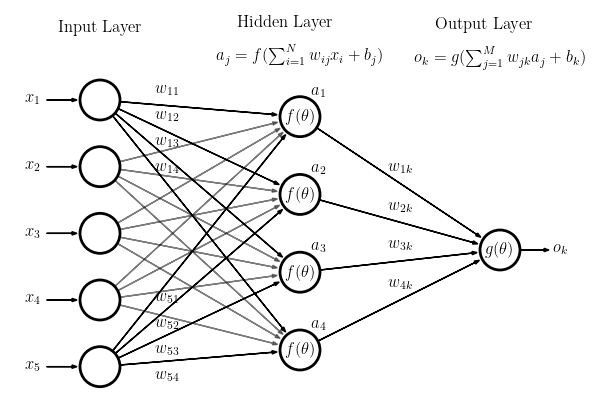
\includegraphics[scale=0.5]{dl.png}\\
        \caption{Example of a deep neural network}
        \label{fig:dl}
    \end{figure}
\end{frame}

\begin{frame}{Backpropogation}
    By doing backpropogation on each node, we finish the process. 
    \begin{figure}
        \centering
        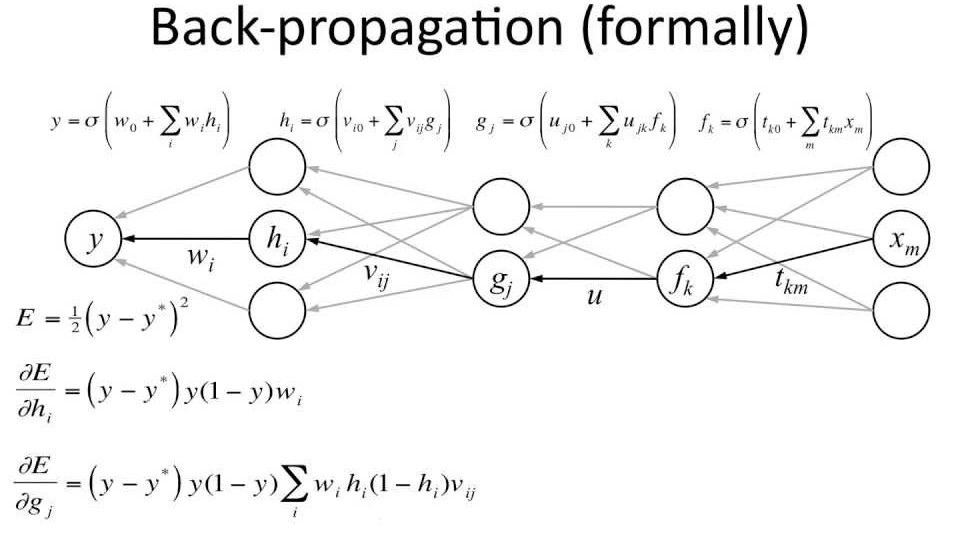
\includegraphics[scale=0.25]{bp.jpg}\\
        \caption{Example of backpropogation }
        \label{fig:bp}
    \end{figure}
\end{frame}

\begin{frame}{Reinforcement Learning}
    What is reinforcement learning? How is it different from supervised and unsupervised learning?
    \begin{figure}
        \centering
        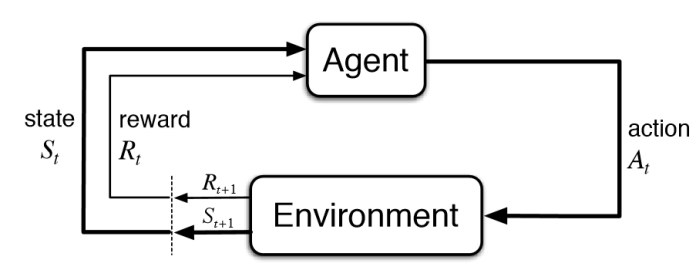
\includegraphics[scale=0.5]{rl.jpg}\\
        \caption{Example of a framework of a reinforcement learning agent }
        \label{fig:rl}
    \end{figure}
\end{frame}

\begin{frame}[fragile]{Value Iteration}
    \begin{lstlisting}[language=python, caption=value iteration algorithm]
    for s in S:
        V(s)=0
    while(not converged):
        for s in S:
            V(s)=R(s)+max over all action[gamma*(sum(P(s,a,s')V(s')))]
    \end{lstlisting}
\end{frame}

\begin{frame}[fragile]{Policy Iteration}
\begin{lstlisting}[language=python, caption=Policy iteration algorithm]
initialize random pi
while(not converged):
    V=V(pi)
    for s in S:
        pi(s)=max over all actions[sum(P(s,a,s')V(S'))]
\end{lstlisting}
\end{frame}

\begin{frame}{Deep Reinforcement Learning}
    Deep reinforcement learning combines Deep learning and reinforcement learning
    \begin{figure}
        \centering
        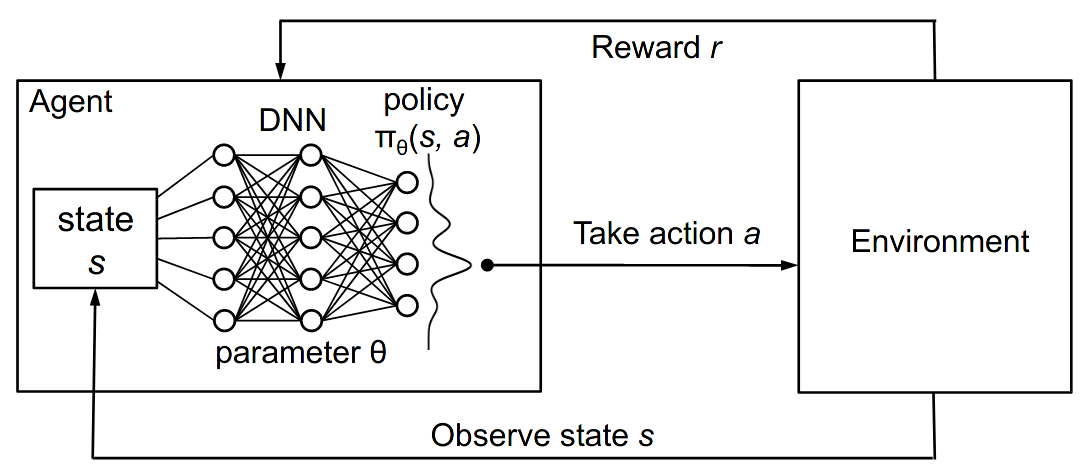
\includegraphics[scale=0.25]{drl.png}\\
        \caption{Deep Reinforcement learning(DQN) framework}
        \label{fig:drl}
    \end{figure}
\end{frame}
